%%%%%%%%%%%%%%%%%%%%%%%%%%%%%%%%%%%%
% Slide options
%%%%%%%%%%%%%%%%%%%%%%%%%%%%%%%%%%%%

% Option 1: Slides with solutions

\documentclass[slidestop,compress,mathserif]{beamer}
\newcommand{\soln}[1]{\textit{#1}}
\newcommand{\solnGr}[1]{#1}

% Option 2: Handouts without solutions

%\documentclass[11pt,containsverbatim,handout]{beamer}
%\usepackage{pgfpages}
%\pgfpagesuselayout{4 on 1}[letterpaper,landscape,border shrink=5mm]
%\newcommand{\soln}[1]{ }
%\newcommand{\solnGr}{ }

%%%%%%%%%%%%%%%%%%%%%%%%%%%%%%%%%%%%
% Style
%%%%%%%%%%%%%%%%%%%%%%%%%%%%%%%%%%%%

\input{../../lec_style.tex}


%%%%%%%%%%%%%%%%%%%%%%%%%%%%%%%%%%%%
% Preamble
%%%%%%%%%%%%%%%%%%%%%%%%%%%%%%%%%%%%

\title[Chp 1: Intro. to data]{Chapter 1: Introduction to data}
\author{OpenIntro Statistics, 4th Edition}
\institute{$\:$ \\ {\footnotesize Slides developed by Mine \c{C}etinkaya-Rundel of OpenIntro. \\
The slides may be copied, edited, and/or shared via the \webLink{http://creativecommons.org/licenses/by-sa/3.0/us/}{CC BY-SA license.} \\
Some images may be included under fair use guidelines (educational purposes).}}
\date{}

%%%%%%%%%%%%%%%%%%%%%%%%%%%%%%%%%%%%
% Begin document
%%%%%%%%%%%%%%%%%%%%%%%%%%%%%%%%%%%%

\begin{document}


%%%%%%%%%%%%%%%%%%%%%%%%%%%%%%%%%%%%
% Title page
%%%%%%%%%%%%%%%%%%%%%%%%%%%%%%%%%%%%

{
\addtocounter{framenumber}{-1} 
{\removepagenumbers 
\usebackgroundtemplate{\includegraphics[width=\paperwidth]{../../OpenIntro_Grid_4_3-01.jpg}}
\begin{frame}

\hfill \includegraphics[width=20mm]{../../oiLogo_highres}

\titlepage

\end{frame}
}
}


%%%%%%%%%%%%%%%%%%%%%%%%%%%%%%%%%%%%
% Sections
%%%%%%%%%%%%%%%%%%%%%%%%%%%%%%%%%%%%

%%%%%%%%%%%%%%%%%%%%%%%%%%%%%%%%%%%%
\section{Course Introduction}
%%%%%%%%%%%%%%%%%%%%%%%%%%%%%%%%%%%%

% TODO: in lecture? using Edfinity, Pronto, or something else?
\begin{frame}
	\frametitle{Class poll/discussion board: Getting to know you!}

	\begin{itemize}
		\item What has your past experience in Statistics been, if any? What about other math courses?
		\item What are your interests? (These may help inform lab activities and lecture examples!)
		\item For group projects in labs, how would you prefer groups be formed?
		\item What are your goals for the course?
	\end{itemize}
\end{frame}

\begin{frame}
	\frametitle{Course Information and Syllabus}
\end{frame}

%%%%%%%%%%%%%%%%%%%%%%%%%%%%%%%%%%%%

\section{Jumping in: Data basics}

%%%%%%%%%%%%%%%%%%%%%%%%%%%%%%%%%%%%

\subsection{Observations and variables}

\begin{frame}
\frametitle{Classroom survey}

A survey was conducted on students in an introductory statistics course. Below are a few of the questions on the survey, and the corresponding variables the data from the responses were stored in:

\begin{itemize}
\item \var{gender}: What is your gender? 
\item \var{intro\_extra}: Do you consider yourself introverted or extraverted? 
\item \var{sleep}: How many hours do you sleep at night, on average?
\item \var{bedtime}: What time do you usually go to bed?
\item \var{countries}: How many countries have you visited?
\item \var{dread}: On a scale of 1-5, how much do you dread being here?
\end{itemize}

\end{frame}

%%%%%%%%%%%%%%%%%%%%%%%%%%%%%%%%%%%%

\begin{frame}
\frametitle{Data matrix}

Data collected on students in a statistics class on a variety of variables:

\begin{center}
\begin{tabular}{l cccc l}
		& \hl{variable} \\
		& \hl{$\downarrow$}	 \\
\cline{1-5}
Stu.	&	\var{gender}	&	\var{intro\_extra} & $\cdots$ & \var{dread} \\
\cline{1-5}
1 & male   & extravert  & $\cdots$  & 3 \\ 
2 & female & extravert  & $\cdots$  & 2 \\ 
3 & female & introvert  & $\cdots$  & 4 & \hl{$\leftarrow$}  \\ 
4 & female & extravert  & $\cdots$  & 2 & \hl{observation} \\
$\vdots$	 &	$\vdots$	&	$\vdots$  &	$\vdots$ &	$\vdots$ \\
86	& male & extravert  & $\cdots$  & 3 \\
\cline{1-5}
\end{tabular}
\end{center}

\end{frame}

%%%%%%%%%%%%%%%%%%%%%%%%%%%%%%%%%%%%

\subsection{Types of variables}

\begin{frame}
\frametitle{Types of variables}

\begin{center}
%\includegraphics[width=0.9\textwidth]{1-2_data_basics/figures/variables/variables}
\end{center}

\end{frame}

%%%%%%%%%%%%%%%%%%%%%%%%%%%%%%%%%%%

\begin{frame}
\frametitle{Types of variables (cont.)}

\begin{center}
{\footnotesize
\begin{tabular}{c ccc cc}
  \hline
 & \var{gender} & \var{sleep} & \var{bedtime} & \var{countries} & \var{dread} \\
  \hline
1 & male & 5 & 12-2 & 13 & 3 \\ 
  2 & female & 7 & 10-12 & 7 & 2 \\ 
  3 & female & 5.5 & 12-2 & 1 & 4 \\ 
  4 & female & 7 & 12-2 &  & 2 \\ 
  5 & female & 3 & 12-2 & 1 & 3 \\ 
  6 & female & 3 & 12-2 & 9 & 4 \\ 
  \hline
\end{tabular}
}
\end{center}

\begin{itemize}
\item \var{gender}: \pause \soln{\only<2->{categorical}} \pause
\item \var{sleep}: \pause \soln{\only<4->{numerical, continuous}} \pause
\item \var{bedtime}: \pause \soln{\only<6->{categorical, ordinal}} \pause
\item \var{countries}: \pause \soln{\only<8->{numerical, discrete}} \pause
\item \var{dread}: \pause \soln{\only<10->{categorical, ordinal - could also be used as numerical}}
\end{itemize}

\end{frame}

%%%%%%%%%%%%%%%%%%%%%%%%%%%%%%%%%%%

% \begin{frame}
% \frametitle{Practice}

% \pq{What type of variable is a telephone area code?}

% \begin{enumerate}[(a)]
% \item numerical, continuous
% \item numerical, discrete
% \solnMult{categorical}
% \item categorical, ordinal
% \end{enumerate}

% \end{frame}

%%%%%%%%%%%%%%%%%%%%%%%%%%%%%%%%%%%

\subsection{Relationships among variables}

%%%%%%%%%%%%%%%%%%%%%%%%%%%%%%%%%%%

\begin{frame}
\frametitle{Relationships among variables}

\dq{Does there appear to be a relationship between GPA and number of hours students study per week?}

\begin{center}
%\includegraphics[width=0.7\textwidth]{1-2_data_basics/figures/gpa_study_hours/gpa_study_hours}
\end{center}

\pause

\dq{Can you spot anything unusual about any of the data points?}

\soln{\pause{There is one student with GPA $>$ 4.0, this is likely a data error.}}

\end{frame}

%%%%%%%%%%%%%%%%%%%%%%%%%%%%%%%%%%%

\subsection{Explanatory and response variables}

%%%%%%%%%%%%%%%%%%%%%%%%%%%%%%%%%%%

\begin{frame}
\frametitle{Explanatory and response variables}

\begin{itemize}

\item To identify the explanatory variable in a pair of variables, identify which of the two is suspected of affecting the other:

\begin{center}
explanatory variable $\xrightarrow{might~affect}$response variable
\end{center}

\item Labeling variables as explanatory and response does not guarantee the relationship between the two is actually causal, even if there is an association identified between the two variables. We use these labels only to keep track of which variable we suspect affects the other.

\end{itemize}

\end{frame}

%%%%%%%%%%%%%%%%%%%%%%%%%%%%%%%%%%%

\subsection{Introducing observational studies and experiments}

%%%%%%%%%%%%%%%%%%%%%%%%%%%%%%%%%%%

\begin{frame}
\frametitle{Two primary types of data collection}

\begin{itemize}

\item \hl{Observational studies:} Collect data in a way that does not directly interfere with how the data arise (e.g. surveys).
\begin{itemize}
\item Can provide evidence of a naturally occurring association between variables, but they cannot by themselves show a causal connection.
\end{itemize}

\pause

\item \hl{Experiment:} Researchers randomly assign subjects to various treatments in order to establish causal connections between the explanatory and response variables.


\end{itemize}

\end{frame}

%%%%%%%%%%%%%%%%%%%%%%%%%%%%%%%%%%%

\begin{frame}
\frametitle{Association vs. causation}

\begin{itemize}

\item When two variables show some connection with one another, they are called \hl{associated} variables.
\begin{itemize}
\item Associated variables can also be called \hl{dependent} variables and vice-versa.
\end{itemize}

\item If two variables are not associated, i.e. there is no evident connection between the two, then they are said to be \hl{independent}.

\item In general, association does not imply causation, and causation can only be inferred from a randomized experiment.

\end{itemize}

\begin{center}
%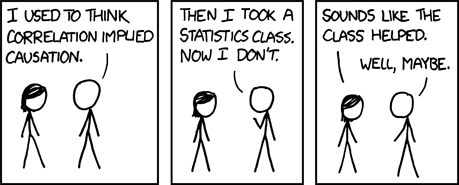
\includegraphics[width=0.55\textwidth]{1-2_data_basics/figures/xkcd_correlation} \\
{\tiny \webURL{http://xkcd.com/552/}}
\end{center}

\end{frame}

%%%%%%%%%%%%%%%%%%%%%%%%%%%%%%%%%%%%

% \begin{frame}
% \frametitle{Practice}

% \twocol{0.5}{0.5}
% {
% \pq{Based on the scatterplot on the right, which of the following statements is correct about the head and skull lengths of possums?}
% }
% {
% %\includegraphics[width=\textwidth]{1-2_data_basics/figures/possum_head_skull/possum_head_skull}
% }

% \begin{enumerate}[(a)]
% \item There is no relationship between head length and skull width, i.e. the variables are independent.
% \solnMult{Head length and skull width are positively associated.}
% \item Skull width and head length are negatively associated.
% \item A longer head causes the skull to be wider.
% \item A wider skull causes the head to be longer.
% \end{enumerate}

% \end{frame}

%%%%%%%%%%%%%%%%%%%%%%%%%%%%%%%%%%%

\section{Edfinity quiz}

%%%%%%%%%%%%%%%%%%%%%%%%%%%%%%%%%%%

%%%%%%%%%%%%%%%%%%%%%%%%%%%%%%%%%%%%
% End document
%%%%%%%%%%%%%%%%%%%%%%%%%%%%%%%%%%%%

\end{document}